
\documentclass[journal]{IEEEtran}

\usepackage[utf8]{inputenc}

\ifCLASSINFOpdf
   \usepackage[pdftex]{graphicx}
   
  % declare the path(s) where your graphic files are
  % \graphicspath{{../pdf/}{../jpeg/}}
  % and their extensions so you won't have to specify these with
  % every instance of \includegraphics
   \DeclareGraphicsExtensions{.pdf,.jpeg,.png}
\else
  % or other class option (dvipsone, dvipdf, if not using dvips). graphicx
  % will default to the driver specified in the system graphics.cfg if no
  % driver is specified.
  % \usepackage[dvips]{graphicx}
  % declare the path(s) where your graphic files are
  % \graphicspath{{../eps/}}
  % and their extensions so you won't have to specify these with
  % every instance of \includegraphics
  % \DeclareGraphicsExtensions{.eps}
\fi

\ifCLASSOPTIONcompsoc
 \usepackage[caption=false,font=normalsize,labelfont=sf,textfont=sf]{subfig}
\else
 \usepackage[caption=false,font=footnotesize]{subfig}
\fi


\hyphenation{op-tical net-works semi-conduc-tor}


\begin{document}

\title{Bare Demo of IEEEtran.cls\\ for IEEE Journals}


\author{Isaac~Sacramento,
        Elton~Trindade,
        Mauro~Roisenberg,
        Fernando~Bordignon,
        and~Bruno~Rodrigues
\thanks{I. Sacramento and M. Roisenberg are with the Departament of Computer Science, Informatics and Statistics Institute,
Federal University of Santa Catarina, Florianópolis, Santa Catarina, Brazil (e-email: isaac.sacramento@posgrad.ufsc.br;
mauro.roisenberg@ufsc.br).}% <-this % stops a space
\thanks{E. Trindade is with Petrobras, Rio de Janeiro, Rio de Janeiro, Brazil (e-email: elton.trindade@petrobras.com.br).}% <-this % stops a space
\thanks{F. Bordignon is with Cognitive and Connectionism Laboratory, Federal University of Santa Catarina, Florianópolis,
Santa Catarina, Brazil (e-mail: f.bordignon@gmail.com).}
\thanks{B. Rodrigues is with Petrobras, Rio de Janeiro, Rio de Janeiro, Brazil (e-email: bbrodrigues@gmail.com).}}

% The paper headers
\markboth{Journal of \LaTeX\ Class Files,~Vol.~14, No.~8, August~2015}%
{Shell \MakeLowercase{\textit{et al.}}: Bare Demo of IEEEtran.cls for IEEE Journals}

\maketitle

\begin{abstract}
Domain-specific methods for deblurring particular sorts of
objects have gained increasing attention due to the ineffectiveness
of generic methods.
We present a simple and effective convolutional
neural network that deblurs post-inversion acoustic impedance images. 
The architecture of our model consists of a convolutional layer
that highlight edges and contours related to
interfaces between rock layers; a locally-connected
layer, that performs a convolutional step with unshared weights;
finally, two fully-connected layers that
perform a non-linear estimation of acoustic impedance values.
We use the updated Standford VI reservoir model as training dataset,
which is composed of 200 acoustic impedance sections, each section with
150 traces. In our work, we adopt a strong supervised learning
that exploit, trace by trace, the dataset of the inverted and ground truth impedance images.
We also present an analysis comparing the frequency band-width among 
the latent, blurry, and deblurred images. Furthermore, the Signal-to-Noise Ratio (SNR)
is calculated and compared with a classical deblurring method.
We additionally address the requirement of deep learning for the huge amount
of training examples by inserting rectified linear units (ReLU) and keeping
the network architecture simple. 
The experimental results demonstrate the efficacy of the proposed method.
\end{abstract}

% Note that keywords are not normally used for peerreview papers.
\begin{IEEEkeywords}
convolutional neural network, acoustic impedance, deblurring, seismic inversion, frequency recovering.
\end{IEEEkeywords}

\IEEEpeerreviewmaketitle



\section{Introduction}

\IEEEPARstart{T}{his} letter presents a deep convolutional
approach for recovering high frequency components in
post-inversion acoustic impedance models. The inversion of
seismic data to obtain acoustic impedance is a frequently
used technique because it offers several advantages: (1) it
facilitates integrated interpretation, (2) stochastic
inversion can improve data's vertical resolution, allowing
sub-seismic features to be more precisely mapped, and (3)
it optimizes the correlation between seismic and petrophysical
properties of the reservoir. However, using the seismic data in
deep-water reservoir modeling leads to errors in estimating
the reservoir properties because such data do not allow the
wider understanding of the field under study \cite{Sergio2016}.

The seismic vertical resolution is the minimal thickness that
can be resolved by seismic. The most accepted value is a quarter
of the wave length, that means that only layers thicker than
that will be detected by seismic acquisition. In larger depths
that value can be as high as $20$ meters, which may represent a
significant amount of oil volume being under or overestimated.
%or mitigate connectivity problems.
Even though the inversion
process can add low frequencies to the acoustic impedance
spectrum through a constraint model, results from a typical
post-stack or pre-stack seismic inversion are band-limited
primarily due to missing very low and high frequencies in the
wavelet. Consequently, thin beds are generally poorly resolved
\cite{Zhang2012}. The limited vertical resolution in the
conventional seismic data is due to the limited frequency of
the data in both low frequencies and high frequencies.

In deterministic inversion approaches, the vertical resolution
remains constrained by the seismic bandwidth \cite{Sancevero2005}.
Deterministic inversion is mainly useful for deriving general
trends and highlighting large features in an exploratory stage.
On the other hand, stochastic inversion uses random variation
of parameters to reach results with vertical resolution that is
superior to the conventional data. When working with multiple
realizations, selecting the model that best characterizes the
reservoir is difficult, since all of them are equally probable.
Uniqueness problems are an issue mainly addressed by calculating
the mean of different realizations. However, it has been proved
that the mean solution is closer to a bandwidth limited solution,
in such a way that the high frequencies features are lost
\cite{Cook2010}. An approach to deal with the high frequency
impedance information out of the frequency bandwidth of seismic signal
is assuming a blocked model for the earth's impedance \cite{Cook2010}.
This assumption is not always valid, and in some cases the high
frequencies in the inverted impedance are ignored \cite{YuanWang2015}.
\cite{xiaoiu} aim to enhance the seismic acquisition resolution and, by
consequence, achieving an improvement in seismic inversion and
reservoir characterization, while \cite{ChenWang2018} latest use wavelet
frequency-dependent scaling to extends the amplitude spectrum of
high and low-frequency axes in time domain. 
%However, the earth
%attenuation, high-frequency noise and other sources cause the lack of high and
%low frequencies in seismic data.

% giving the result of the inversion process a blurry aspect that
% makes unfeasible visualizing thin beds
In this letter, we propose a new multichannel and multilayer
Convolutional Neural Network (CNN) model to perform deblurring
in post-inversion acoustic impedance. Each network's layer maps
higher level features originating in the previews layers through
one-dimensional convolutional blur kernels. To perform this
mapping, the kernels (also named weights) are adjusted by
minimizing a loss function. The model enhances the resolution
of acoustic impedance images trace by trace, resulting in sharper
images with increased high-frequency bandwidth and lower noise.
In order to train the model, we perform \textit{Maximum-a-Posteriori} (MAP)
inversion that commonly generates a band-limited acoustic impedance model.
Then, the pairs of blurry and latent images are normalized and 
presented to the network as input and target, respectively.
<<<<<<< HEAD
The core concept of our architecture is the combination of the
convolutional, locally-connected and regression layers. Thus
the convolutional layer learns the spatial structures existing
in different acoustic impedance images, the locally-connected
layer individualizes and refines the resolution of these structures,
finally, the regression layer proceeds the prediction of the property values.
Thus, deblurring the acoustic impedance models, as a post-inversion
refinement process, should lead to a more accurate interpretation
of the impedance models.

The contributions of this work are threefold. First,
according to our knowledge, it is the first to approach
inversion resolution enhancement through a post-inversion
refinement. Second, the proposed deep learning model
effectively recovers the high frequency spectrum absent
in the post-inversion acoustic impedance. Additionally, it
corrects deformations existing in thin bodies caused
by the inversion process. Third, our proposal
shows to be more embracing than the state-of-art
methods, since the CNN learns the high frequency
based on different possible scenarios and freely solve
the occurrences in the post-inversion images.

The remainder of this letter is organized as follows.
Section \ref{Theoretics} reviews the deblurring methods
and the CNN, a popularly used deep-learning technique.
Section \ref{Method} describes the data and used for
training the CNN and the architecture of the proposed model.
Section \ref{Experiments} reports the experiments and
results, and Section \ref{Conclusion} concludes our work.
=======
In our approach, the domain-specific knowledge used in deblurring acoustic impedance impedance images is commonly
obtained through training images containing geological knowladge. Generally, the images are obtained from a specialist's
(geologist or geophysicist) knowledge about relevant characteristics of the reservoir for which one wishes enhancing the impedance images.
The core concept of our architecture is the combination of the convolutional layers with regression layers, thus the convolutional layers learn the spatial structures existing in different acoustic impedance images, while the regression layer proceed the prediction of the property values.

Thus, deblurring the acoustic impedance models, as a post-inversion refinement process, should lead to a more accurate
interpretation of the impedance models.

The remainder of this letter is organized as follows. Section II
reviews the CNN, a popularly used deep-learning technique.
Section III describes the proposed deblurring approach.
Section IV \ref{Theoretics} reports the experiments and results, and Section \ref{Theoretics}
concludes our work.

% % \hfill mds
% %  
% % \hfill August 26, 2015


>>>>>>> 2dd7b352d7f20ab78d8a5c8717fb3ddef405c9dc
% needed in second column of first page if using \IEEEpubid
%\IEEEpubidadjcol

\section{Theoretical Foundations and Related Works}\label{Theoretics}

Deblurring is generally modeled as the convolution of a blur kernel $k$
with a latent image $I$: 
\begin{equation}
 y = k \otimes I + n
 \label{eq:deblurr}
\end{equation}
where $n$ is the noise. Since $k$, $I$ and $n$ are unknown, the problem 
is highly ill-posed and admits infinite solutions for $k$ and $I$.
Blind deconvolution refers to the inference of the sharp image $I$,
given only the blurry image $y$, without any knowledge regarding the
kernel $k$ and the noise $n$ \cite{Zhang2013}. In contrary, if $k$
is assumed to be known, the approach is called non-blind deconvolution
\cite{Wang2009}.
%Several works have developed different deblurring methods
%for specific purposes. For the last six years, considerable effort has
%been made in single image \cite{Babacan2012,Krishnan2015,Levin2011,Zhang2011}
%and multi-image \cite{sroubek2012,Zhu2012} blind deconvolutions.
Applying blind deconvolution generally implies in making assumptions
on blur kernels and/or on latent images. For example, assuming sparsity
of blur kernel or that natural images have super-Gaussian statistics.
The second assumption leads to the use of image priors on inference process
and, consequently, to the maximum \textit{a posteriori} (MAP) estimation
\cite{Babacan2012}. However, \cite{Levin} show that deblurring methods based
on this prior tend to favor blurry images over original latent images.

The Bayesian inference approach \cite{Levin} outperforms the MAP based
methods. It marginalizes the image from the optimization step, while
estimating the unknown blur. 
%The authors show that it is possible to
%define a class of prior images based on natural image statistics,
%suitable enough to represent sharp images features. This prior
%formulation makes possible to use Bayesian inference in the
%estimation of the unknown image and the blur kernel.
According to \cite{Hacohen13}, defining a gradient prior, by itself,
is not sufficient to reach a sharp image, instead, they search in a data
set for a prior that densely correspond to the blurry image similar
to a sharp image. Even though \cite{Pan2014} suggest a generalization
for the method proposed by \cite{Hacohen13}, it still requires a similar
reference image, which is not always available.

%It has been demonstrated that 
The methods described previously fail when applied to real world
blurry images \cite{Lai2016} and take a severe computational cost
\cite{Chakrabarti2016}. In contrast, the learning-based methods
have gained attention with the resumption and recent advances in
convolutional neural networks (CNN). 
Currently, CNN is one of the most successful methods in computer vision.
A basic architecture of a CNN model is composed of a convolutional layer
with non-linear activation neuron, and a pooling layer.
The convolutional layer takes into account a fixed-size and spacial
location portion of the previous layer, and outputs
a weighted representation of its input.
Pooling layers calculate statistical summaries of spatial dimensions
to down-sample feature maps. Thus, pooling layers can extract
contextual information from a larger spatial context.

The adequate hyper-parameter adjustment allows CNN to learn non-linear
function or blur kernels. Thus, deblurring becomes a function of
a blurry image $I$ and a set of parameters $p$ as \ref{eq:deblur}
\begin{equation}
 y = \sigma(I,p)
 \label{eq:deblur}
\end{equation}
Learning-based methods focus on developing a model to learn the function
$\sigma$ and to perform non-blind deblurring \cite{Chakrabarti2016}.
\cite{Sun2015} teaches a CNN to recognize motion kernels and performs non-blind
deconvolution in dense motion field estimate, in addition, \cite{Hradis2015}
minimize regularized $l_2$ in order to perform text deblurring.
In our approach, we perform a blind deconvolution by letting a CNN model
to learn the unknown kernels that best deblurr the acoustic impedance
traces, based on the knowledge of the ground truth image and their
correspondent seismic traces.

\section{Data and Methods}\label{Method}

\subsection{Proposed Architecture}

We propose a four-layer multichannel CNN architecture for deblurring
post-inversion acoustic impedance images and recovering high
frequency of thin layers. The model takes in each input channel the
blurry acoustic impedance trace and the respective seismic
profile. Additionally, by using the ground truth AI trace as
target, the network is able to learn with the acoustic
impedance data in association with the local high frequency seismic.
The model consists of one convolutional layer and one locally-connected
layer, each one of them followed by max pooling. The output of the
locally-connected layer is flatted and two fully connected layers are
added in the end (Fig. \ref{fig_model}).
\begin{figure}[!t]
\centering
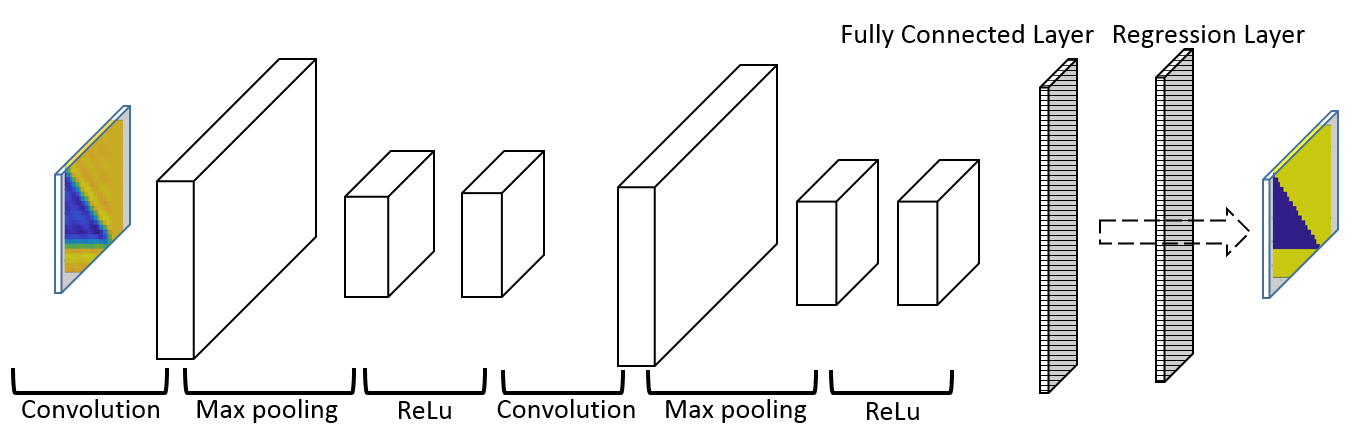
\includegraphics[width=3.4in]{Figs/model}
\DeclareGraphicsExtensions.
\caption{Examples.}
\label{fig_model}
\end{figure}

The first convolutional layer deblurs the lower features in
the input traces. Following, higher features are individually
deblurred through a locally-connected layer \cite{},
which performs a one-dimensional convolution
with unshared weights. Thus, instead of performing standard
convolution, the weights of the learned kernel matrices are not
shared across the input. The number of filters in the convolution
and locally-connected layers is $50$ and $100$, respectively.
As long as the number of filters increases from the first to the
second layer, the size of each filter decreases from $20$ to $10$.
This way, we note that the CNN learns thinner geological
bodies in the second layer.

We use rectified linear unit (ReLU) function that is one
of the most popular and efficient activation functions for
CNNs. There are advantages of using ReLU such as efficient
computation, and gradient propagation. The network uses
Adam to optimize the loss function. This algorithm
combines the AdaGrad and RMSProp methods and converges more efficiently in
comparison to gradient descent, stochastic gradient descent, AdaGrad
and RMSProp \cite{Kingma2014}. The Mean Absolute Error (MAE) is the
loss function minimized in the training process.

\subsection{Data Set}
To evaluate the proposed deblurring method, an acoustic
impedance data set is collected. \footnote{Available at https://github.com/SCRFpublic/Stanford-VI-E/tree/master/Acoustic\%20Impedance} %Badbox aqui
The data set contains a cube of acoustic impedance values
from the updated Stanford VI reservoir \cite{Lee2012}, which
is represented by a three-dimensional regular stratigraphic
model. The cube contains 150x200x200 cells and the dimensions
of each cell are $25$ meters horizontally and $1$ meter vertically.
The model represents a fluvial channel system composed of three
layers: the lowest one represents deltaic deposits (layer 3), the
middle layer represents meandering channels (layer 2) and the highest
layer (layer 1) sinuous channels, deposited in the fluvial channel system.
\footnote{See \cite{Castro2005} for more details about methodologies and model parameters.}
Some sample images from Stanford VI are shown in Fig. \ref{fig_examples}
% \begin{figure}[!t]
% \centering
% 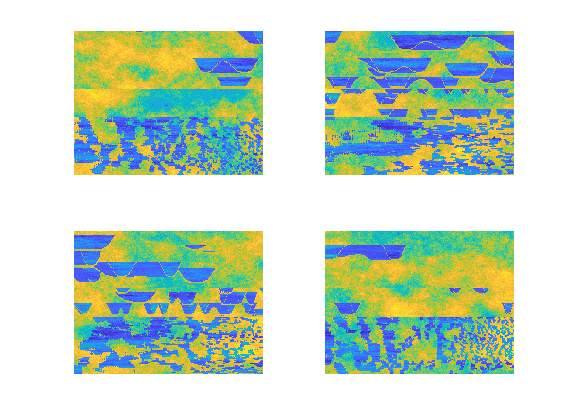
\includegraphics[width=2.5in]{Figs/Examples}
% \DeclareGraphicsExtensions.
% \caption{Examples.}
% \label{fig_examples}
% \end{figure}
Even though the data has been synthetically generated,
the layers represent geological bodies of high importance
in reservoir characterization, such as channels connections and theirs
discontinuity. 

In a realistic scenario, the number of hard data available for
training and validating supervised models is scarce. In order
to address this common issue, we performed experiments with
constrained amount of training data, set to 50\%, 30\% and
10\% of the available data. Using 50\% and 30\% 
produces similar results in the frequency spectrum,
whereas 10\% showed more significant discrepancies in the
amplitude recovering and additional noise mainly in higher frequencies.
(Fig. \ref{fig_imgs}). Therefore, in the following experiments
we adopted 30\% of available data as training data set, once we
observed it is the minimum amount of data to keep the model learning
capability.
\begin{figure}[!t]
\centering
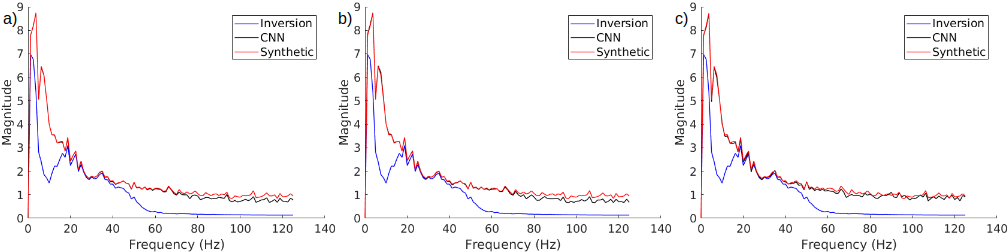
\includegraphics[width=3.5in]{Figs/Images}
\DeclareGraphicsExtensions.
\caption{Examples.}
\label{fig_imgs}
\end{figure}

To build the training data set we carry out the \textit{Maximum-a-Posteriori} (MAP)
\cite{Buland2003,Figueiredo2012} inversion using the high resolution acoustic
impedance. In order to proceed the inversion, we created a Ricker wavelet with
frequency bandwidth from $0Hz$ to $60Hz$, with which the synthetic seismic was
calculated through the forward model. Additionally, a low frequency
model was calculated by applying a low-pass filter with $4Hz$ cutting frequency.
Thus, the \textit{a posteriori} acoustic impedance cube was calculated and the pair of truth
and inverted images compose the training data set. As expected, the inverted
acoustic impedance bandwidth is restricted to the wavelet bandwidth with
addition of the spectrum of the low frequency model. Due to the 1D
convolution adopted in this work, the training data set contains $10000$ trace
samples with $200$ cell along the depth. Each group of $200$ traces composes
a section of the cube.

\section{Experiment and Discussion}\label{Experiments}
Here, we validate the proposed post-inversion deblurring method.
The parameters settings for the model training are presented.
Next, the experimental results are given for the proposed method,
as well as the comparison methods.

\subsection{Model Training}
We will use 33\% (10000 traces)
of the available data, seismic and inverted acoustic impedance traces,
to infer the blur filters. Furthermore, we will adopt 
mini-batches with size of $10$ training examples and exponentially
decreasing learning rate (initially set to $0.001$)
in a total of $150$ iterations.

The network contains two channels in the input layer and we set
each input data in one channel.
It should be noted that every image is different and each
one is introduced only once to the network, this way avoiding
over-fitting. We also deal with this issue by calculating
the loss for the test images, and control the training,
thus we early stop the training as soon as the test loss
stops decreasing (Fig. \ref{}).
Other techniques to avoid over-fitting, such as
drotout, compromised the reconstruction of the entire image.
The network weights
will initialize randomly and the model will perform a supervised
learning over tuples containing the pairs of inverted acoustic
impedance and seismic profile as input, and ground truth traces as targets.
To avoid neuron saturation and still keep the non-linearity predictability
of the CNN, we will normalize the acoustic impedance to values between 0 and 1,
and the results are presented in terms of this normalization.

\subsection{Deblurring Post-Inversion Acoustic Impedance}
By applying the trained model to a set of inverted traces,
we notice that the CNN produced overall shaper acoustic
impedance images. Looking into the details,
the deblurred images show substantial recovery of high frequency events
(thin layers), which can be seen in the intersections between
two channels, as illustrated in Fig. \ref{ImSec26}.
\begin{figure}[!t]
\centering
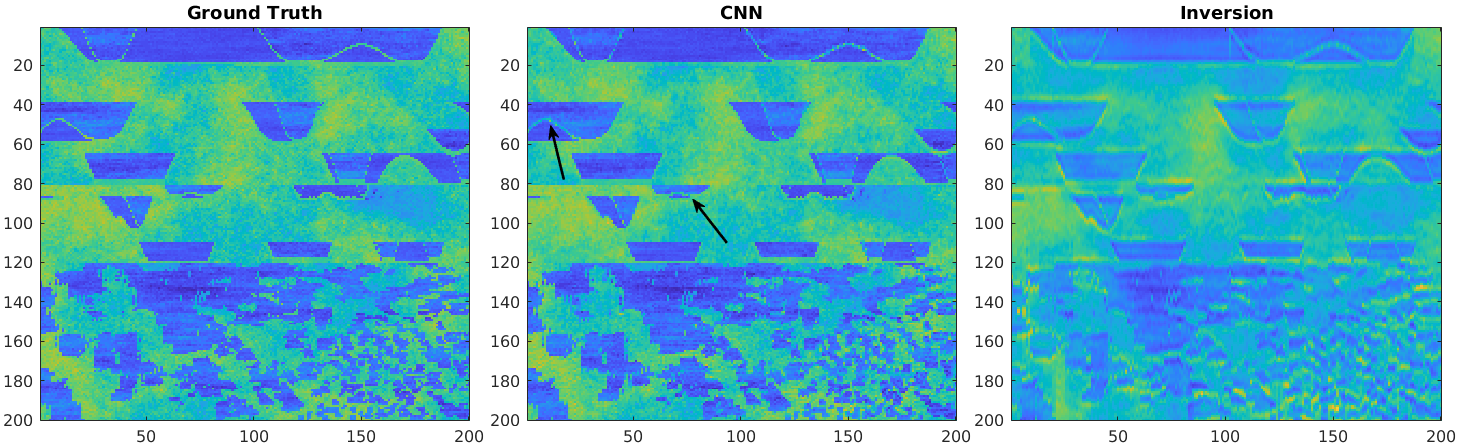
\includegraphics[width=3.5in]{Figs/ImSec26}
\DeclareGraphicsExtensions.
\caption{Examples.}
\label{ImSec26}
\end{figure}

It should be pointed out that the horizontal resolution seem to be
better enhanced when compared to the vertical resolution, which can
be an effect of the wavelet signature and/or the deconvolution process.
The increase in the horizontal resolution is particularly important,
since it is related to events in which the layers become thinner and the porosity
decreases, thus decreases the impedance contrast and, therefore, its
seismic response. The vertical resolution improvement is essential to
evaluate the vertical connectivity in the reservoir. In terms, it is possible
that thin layers of shale act as barriers for the water injection and affect the production
and pressurization of the reservoir. Besides significant improvements
in the resolution, the model managed to correct some geometric deformations
created during the inversion process (Fig. \ref{ImSec36}), which usually
occurs in smaller depositional features, as channels.
\begin{figure}[!t]
\centering
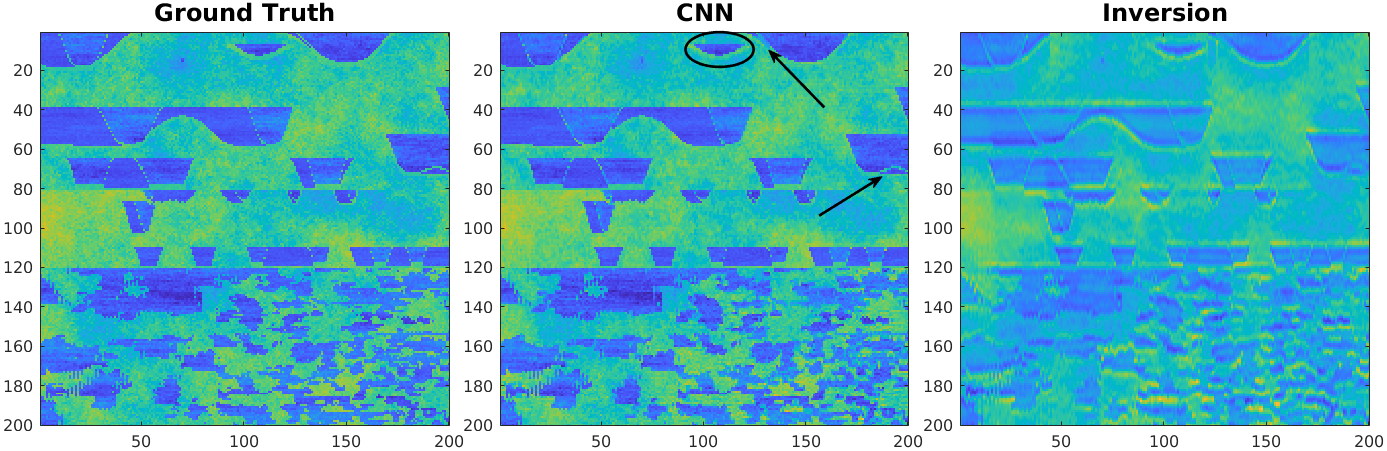
\includegraphics[width=3.5in]{Figs/ImSec36}
\DeclareGraphicsExtensions.
\caption{Examples.}
\label{ImSec36}
\end{figure}

A relevant aspect in deblurring acoustic impedance images
is the observance of high frequencies recovering after the
blurry images being submitted to the CNN. Moreover, the
additional spectrum is associated to the insertion
of high frequency signal, instead of noise.
Fig. \ref{frequencies} introduces the graphs containing the frequency
magnitudes of our test examples, as well as the recovery percentage
for each frequency magnitude. As can be noticed,
the CNN recovered around $100$\% of the signal frequency existing
in the blurry image (from $4Hz$ to $60Hz$). The model recovered
the total frequency in the spectrum lower than
$4Hz$, as long as from $70$ to $90$\% of the possible frequencies
in the spectrum higher than $60Hz$.
Since these ranges of frequencies are absent in the inverted acoustic
impedance, we note that the CNN learned the existing relation between the
seismic profiles and the acoustic impedance in the ground truth images
and correctly rebuilt them in the test images.
\begin{figure}[!t]
\centering
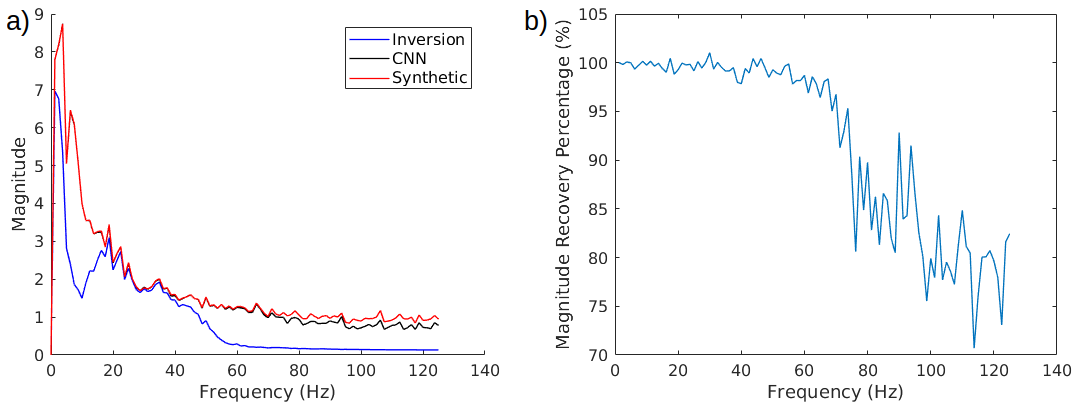
\includegraphics[width=3.5in]{Figs/frequencies}
\DeclareGraphicsExtensions.
\caption{Frequency spectrum comparison between the ground truth image,
the MAP inversion image and the deblurred image. Additionally, the recovery percentage
for each frequency magnitude.}
\label{frequencies}
\end{figure}

In addition, we calculated the Signal-to-Noise Ratio (SNR) of each
test section. Tab. \ref{table_results} list the values of SNR for the
ground truth image, for the result of the inversion method, and
for the image deblurred by the classical method using wiener
filters and by our proposal. The proposed method holds clearly
higher performance than the classical method, since it generates
image with higher SNR. This result endorses that the high frequency
components recovered by the CNN is related to signal, rather than noise.
\begin{table}[!t]
\renewcommand{\arraystretch}{1.3}
\caption{Results evaluated on updated Standford VI reservoir, examples
introduced in Fig. \ref{ImSec26} and Fig. \ref{ImSec36}. Signal-to-Ratio (dB) is listed.}
\label{table_results}
\centering
\begin{tabular}{|c||c||c|}
\hline
 \textbf{Image Section} & \textbf{\textit{Inversion (dB)}} & \textbf{\textit{Wiener Filter (dB)}} & \textbf{\textit{Our (dB)}}\\
\hline
Inline Section& $19.8206$ & $0.1$ & $28.3618$ \\
\hline
Crossline Section& $0.1$ & $0.1$ & $0.1$ \\
\hline
\end{tabular}
\end{table}

\section{Conclusion} \label{Conclusion}
In summary, we proposed a multichannel and multilayer CNN
for post-inversion acoustic impedance deblurring. Moreover, we introduced a simple architecture
that combines convolution, locally connected and regression layers.
We demonstrated that the CNN achieved reasonable results regarding the high frequency
recovering in seismic inversion data. The methodology is promising for deblurring
post-inversion acoustic impedance due to its capability to learn one-dimensional
blur kernels and to recovery two-dimensional geometric features (such as deposition
borders and thin layers). We tested the model on a limited synthetic data set
significantly realistic in its structure and dimensions. 
In order to obtain a more realistic and comprehensive training data, the model
may be fed with shallower portions of the seismic data. This approach is
feasible, since most geological features tend to repeat themselves
(fractal) where the frequency spectrum is broader in the high frequencies (the frequency
amplitude decreases exponentially with depth, due to attenuation and dispersion effects
during propagation).

\section*{Acknowledgment}

The authors would like to thank \textit{Conselho Nacional de Pesquisa e Desenvolvimento,
Fundação de Amparo à Pesquisa e Inovação do Estado de Santa Catarina} and Petrobras
for their support and availability during the work.

\ifCLASSOPTIONcaptionsoff
  \newpage
\fi

\begin{thebibliography}{1}
\bibitem{Sergio2016}
S. S. Sancevero, A. Z. Remacre, R. S. Portugal, "O papel da inversão para a impedância no processo de caracterização sísmica de reservatórios." in Revista Brasileira de Geofísica, p. 495--512, v. 24, 2006.

\bibitem{Zhang2012}
R. Zhang and M. K. Sen and S. Phan and S. Srinivasan, "Stochastic and deterministic seismic inversion methods for thin-bed resolution", Journal of Geophysics and Engineering, V. 9, N. 5, 2012.

\bibitem{Sancevero2005}
S. S. Sancevero and A. Z. Remacre and R. de S. Portugal and E. C. Mundim, "Comparing deterministic and stochastic seismic inversion for thin-bed reservoir characterization in a turbidite synthetic reference model of Campos Basin, Brazil", The Leading Edge, v. 24, num. 11, pp. 1168--1172, 2005. 

\bibitem{Cook2010}
D. Cooke and J. Cant and A. Santos and  P. Wa, Australia,  "Model-based Seismic Inversion: Comparing deterministic and Probabilistic approaches". CSEG Recorder, 2010. 

\bibitem{YuanWang2015}
S. Yuan and S. Wang and C. Luo and Y. He, "Simultaneous multitrace impedance inversion with transform-domain sparsity promotion", Geophysics, pp. 71--80, v. 80, n. 2, 2015.

\bibitem{xiaoiu}
X. Xiaoyu, L. Yun, S. Desheng, G. Xiangyu, and W. Huifeng, "Studying the effect of expanding low or high frequency on post-stack seismic inversion," in SEG Technical Program Expanded Abstracts 2012, pp. 1--5, 2012.

\bibitem{ChenWang2018}
S. Chen and Y. Wang, "Seismic Resolution Enhancement by Frequency-Dependent Wavelet Scaling," in IEEE Geoscience and Remote Sensing Letters, no. 99, pp. 1--5, 2018.

\bibitem{Zhang2013}
H. Zhang, D. Wipf and Y. Zhang, "Multi-image Blind Deblurring Using a Coupled Adaptive Sparse Prior," IEEE Conference on Computer Vision and Pattern Recognition, Portland, OR, pp. 1051--1058, 2013.

\bibitem{Wang2009}
C. Wang, L. Sun, Z. Chen, S. Yang and J. Zhang, "High-quality non-blind motion deblurring," 16th IEEE International Conference on Image Processing (ICIP), Cairo, pp. 153--156, 2009.

\bibitem{Babacan2012}
S. D. Babacan, R. Molina, M. N. Do, and A. K. Katsaggelos, ``Bayesian blind deconvolution with general sparse image priors.'' in Proceedings of European Conference on Computer Vision (ECCV), pp. 341--355, 2012.

\bibitem{Levin}
A. Levin, Y. Weiss, F. Durand, and W. T. Freeman. ``Understanding and evaluating blind deconvolution algorithms.'' In IEEE Proceedings of International Conference on Computer Vision and Pattern Recognition (CVPR), pp. 1964--1971, 2009.

\bibitem{Hacohen13}
Y. Hacohen, E. Shechtman, and D. Lischinski, ``Deblurring by example using dense correspondence.'' In IEEE Proceedings of International Conference on Computer Vision (ICCV), pp. 2384--2391, 2013.

\bibitem{Pan2014}
J. Pan, Z. Hu, Z. Su, and M. H. Yang, ``Deblurring face images with exemplars.'' In Proceedings of European Conference on Computer Vision (ECCV), pp. 47--62. Springer, 2014.

\bibitem{Lai2016}
W.S. Lai, J. B. Huang, Z. Hu, N. Ahuja, and M. H. Yang, ``A comparative study for single image blind deblurring.'' In IEEE Proceedings of International Conference on Computer Vision and Pattern Recognition (CVPR). IEEE, 2016.

\bibitem{Chakrabarti2016}
A. Chakrabarti, ``A neural approach to blind motion deblurring.'' In Proceedings of European Conference on Computer Vision (ECCV), pp. 221--235, Springer, 2016.

\bibitem{Sun2015}
J. Sun, W. Cao, Z. Xu, and J. Ponce, ``Learning a convolutional neural network for non-uniform motion blur removal.'' In IEEE Proceedings of International Conference on Computer Vision and Pattern Recognition (CVPR), pp. 769--777, 2015.

\bibitem{Hradis2015}
M. Hradiš, J. Kotera, P. Zemcı́k, and F. Šroubek, ``Convolutional neural networks for direct text deblurring.'' In Proceedings of British Machine Vision Conference (BMVC), 2015.

\bibitem{Kingma2014}
D. P. Kingma and J. Ba. “Adam: A method for stochastic optimization.” Unpublished paper. [Online]. Available: https://arxiv.org/abs/1412.6980, 2014.

\bibitem{Lee2012}
Lee, J. and Mukerji, T., "The Stanford VI-E reservoir: A synthetic data set for joint seismic-EM time-lapse monitoring algorithms": 25th Annual Report, Stanford Center for Reservoir Forecasting, Stanford University, Stanford, CA, 2012.

\bibitem{Castro2005}
Castro, S., Caers, J., and Mukerji, T., “The Stanford VI reservoir”: 18th Annual Report, Stanford Center for Reservoir Forecasting, Stanford University, Stanford, CA, 2005.

\bibitem{Buland2003}
A. Buland,  and H. Omre, ``Bayesian linearized avo inversion,'' In Geophysics, pp. 185--198, 2003.

\bibitem{Figueiredo2012}
L. P. Figueiredo, M. Santos, M. Roisenberg, G. Neto, and W. Figueiredo, ``Bayesian framework to wavelet estimation and linearized acoustic inversion,'' in Geoscience and Remote Sensing Letters, pp. 1--5, 2012.

\end{thebibliography}

%\begin{IEEEbiography}{Michael Shell}
%Biography text here.
%\end{IEEEbiography}

% if you will not have a photo at all:
%\begin{IEEEbiographynophoto}{John Doe}
%Biography text here.
%\end{IEEEbiographynophoto}


%\begin{IEEEbiographynophoto}{Jane Doe}
%Biography text here.
%\end{IEEEbiographynophoto}

\end{document}


\grid
\grid
